\section{Memory and Execution-Time Profiling}
\label{sec:pmc-results-memory-and-execution-time-profiling}

In this section, we focus on raw memory and execution-time measurements before discussing any modeling approach.
By examining usage patterns, run durations, and dimension-specific behaviors, we contextualize the challenges of predicting peak memory consumption in an \ac{HPC} setting.

\subsection{Linear Trends and Variability}
\label{subsec:linear-trends-and-variability}

Figure~\ref{fig:peak_memory_facet} shows how average peak memory usage tends to scale linearly with the overall volume (\(\text{inlines} \times \text{xlines} \times \text{samples}\)). 
\EB{Para refletir: Daniel, este gráfico por si só já mostra que existe uma relação quase linear entre a feature volume e o consumo de memória destes kernels. Fiquei na dúvida se faz sentido ter toda uma discussão sobre a relação entre as outras features e o consumo de memória depois de já concluir que há uma relação simples (linear) entre a feature volume e consumo de memória.}
The Envelope, \ac{GST3D}, and Gaussian Filter operators each display a relatively direct proportionality between volume and memory demand.
Interestingly, larger volumes produce consistently higher yet less variable memory consumption, whereas smaller volumes display higher \ac{CV}\EBRM{(coefficient of variation)}.

A possible explanation for this disparity is that smaller volumes involve shorter-run processes in which overheads (e.g., Python interpreter initialization, I/O buffering) can appear more prominently, thus creating variability.
As volumes grow, these overheads become negligible compared to the large data arrays and associated computations.
Consequently, memory usage “smooths out” and increasingly reflects the operator’s intrinsic workload characteristics.

\begin{figure*}[htbp]
    \centering
    \begin{subfigure}[t]{0.49\textwidth}
        \centering
        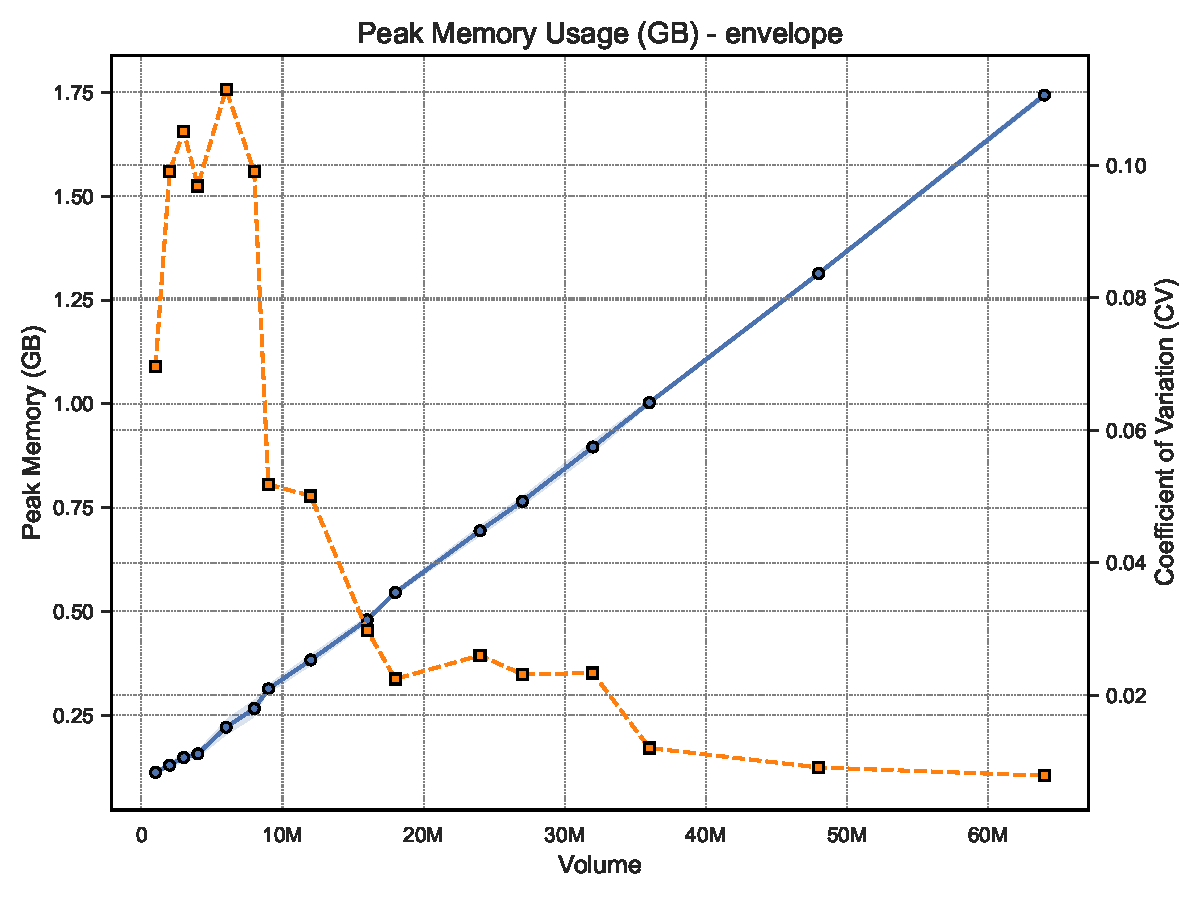
\includegraphics[width=\textwidth]{assets/images/05/peak_memory_by_volume_envelope}
        \caption{Envelope: Smaller volumes exhibit higher variability, while larger volumes show a consistent linear growth trend.}
    \end{subfigure}
    \hfill
    \begin{subfigure}[t]{0.49\textwidth}
        \centering
        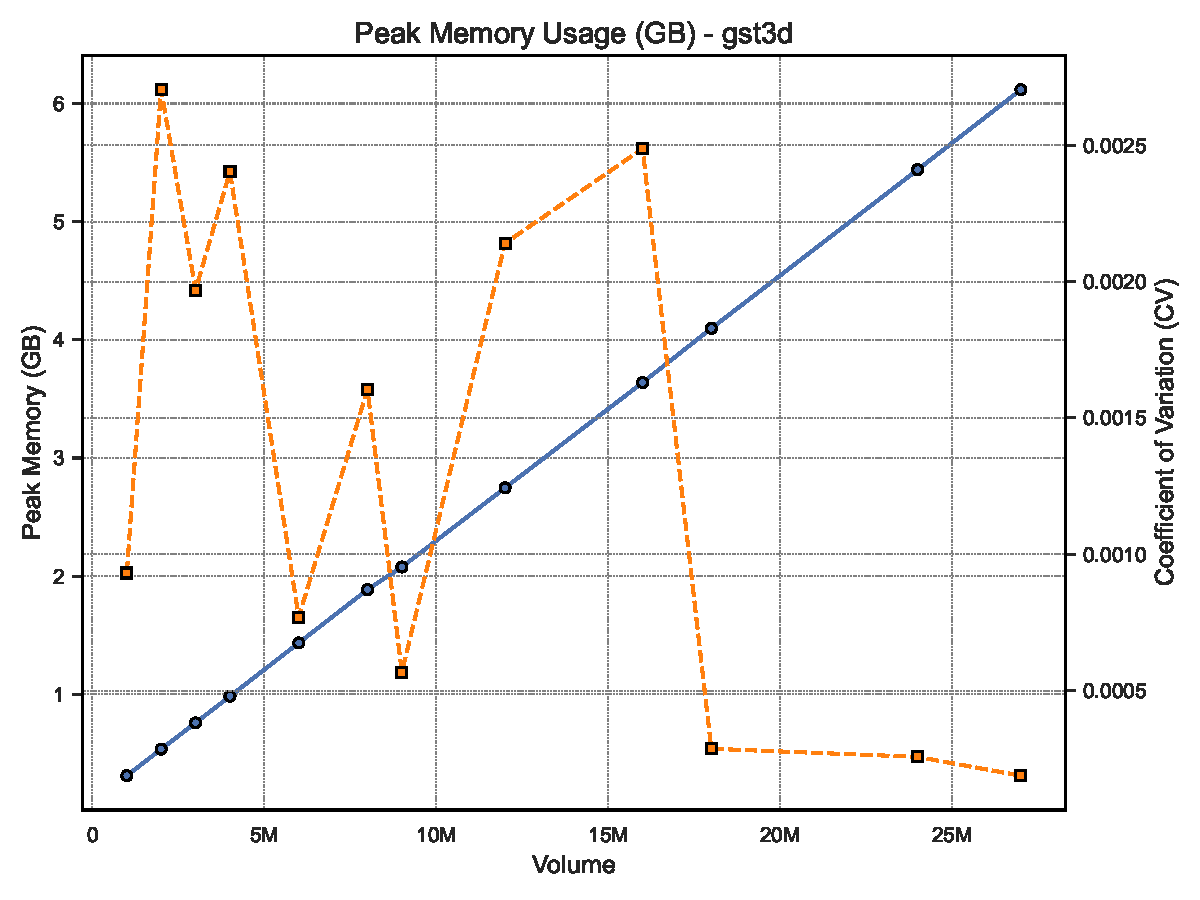
\includegraphics[width=\textwidth]{assets/images/05/peak_memory_by_volume_gst3d}
        \caption{\ac{GST3D}: This operator has a steeper slope compared to Envelope, reflecting more elaborate data structures.}
    \end{subfigure}
    \hfill
    \begin{subfigure}[t]{0.49\textwidth}
        \centering
        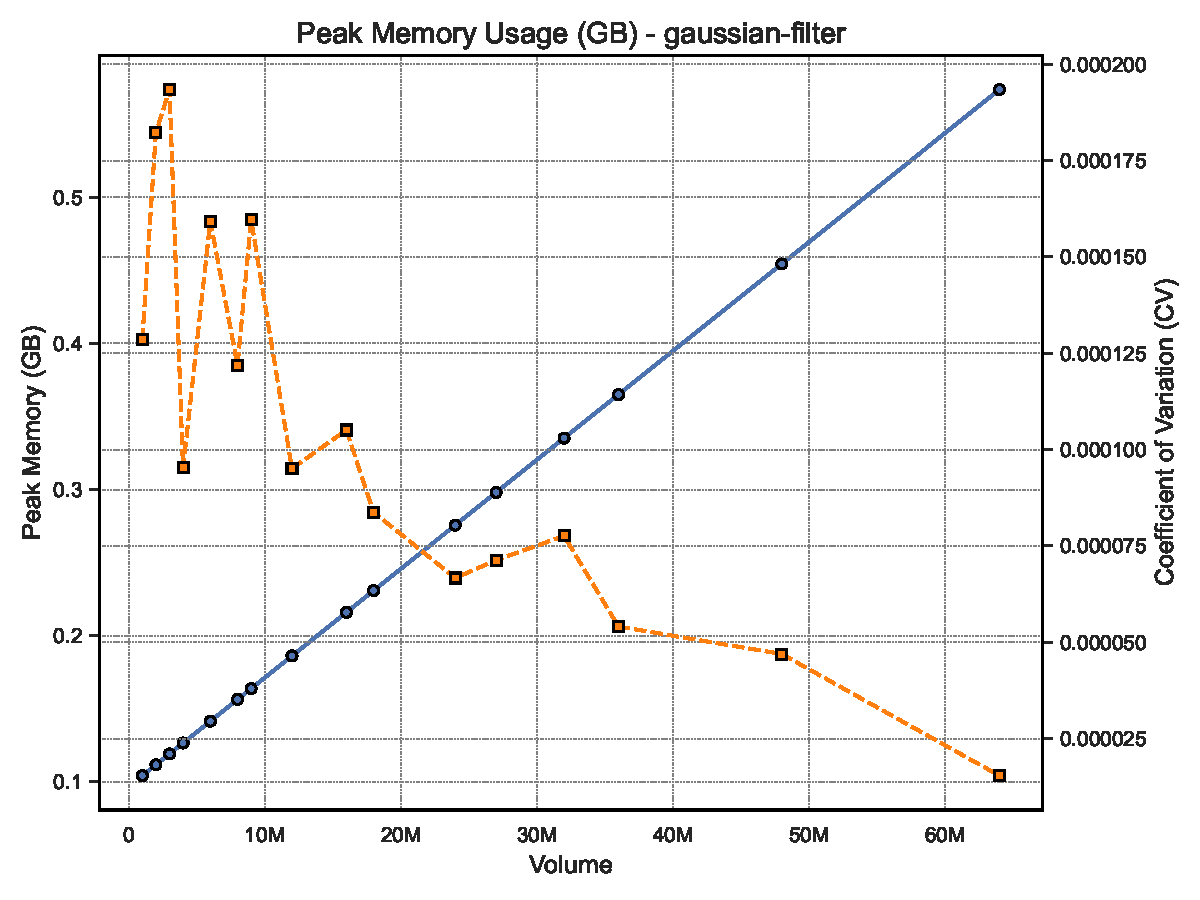
\includegraphics[width=\textwidth]{assets/images/05/peak_memory_by_volume_gaussian-filter}
        \caption{Gaussian Filter: Memory usage also scales linearly but with a gentler slope than \ac{GST3D}.}
    \end{subfigure}
    \caption{Peak memory usage by volume for Envelope, \ac{GST3D}, and Gaussian Filter. 
        Each operator shows an approximate linear growth rate as volume increases, but the slope and variability differ.
        \EB{Verifique se é possível usar o sw gerador de gráficos (matplotlib?) para colocar os três gráficos em uma única linha - um ao lado do outro. Dessa forma, você economizaria bastante espaço e talvez as figuras se encaixem melhor no fluxo do texto -- idealmente a figura deveria vir logo após o parágrafo que referencia ela.}
        \EB{Se possível, também acho que seria legal relembrar o leitor o que significa o termo Volume. Talez usar como rótulo do eixo-x o termo $Volume (inline \times xline \times samples)$}
    }
    \label{fig:peak_memory_facet}
\end{figure*}

In parallel with rising memory usage, Figure~\ref{fig:execution_time_by_volume_facet} (detailed below) confirms that execution times also follow a predominantly linear trajectory with volume.
These combined observations suggest that volume—and more broadly, input shape—acts as a dominant factor in resource demands for \EBRPD{seismic workloads}{these seismic processing kernels}.

\begin{figure*}[htbp]
    \centering
    \begin{subfigure}[t]{0.49\textwidth}
        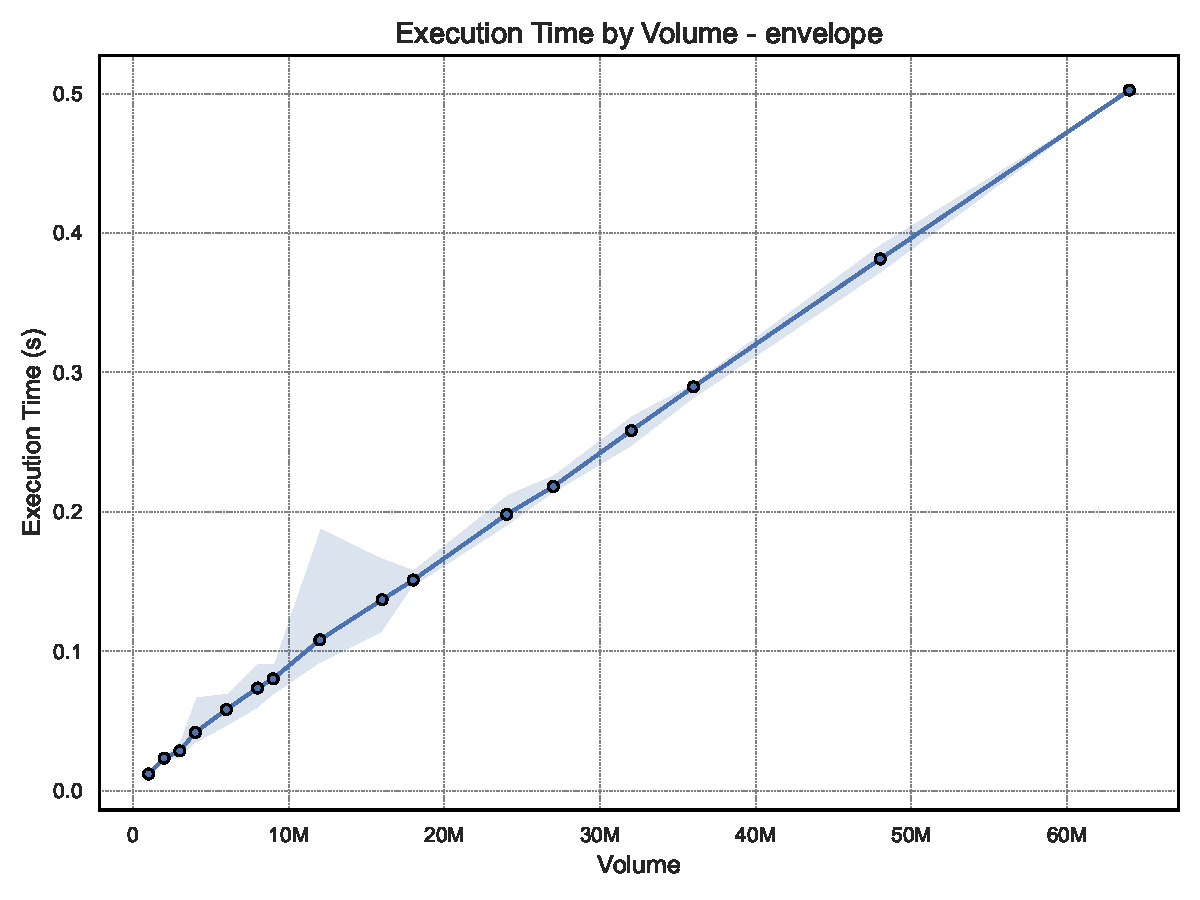
\includegraphics[width=\textwidth]{assets/images/05/execution_time_by_volume_envelope}
    \end{subfigure}
    \hfill
    \begin{subfigure}[t]{0.49\textwidth}
        \centering
        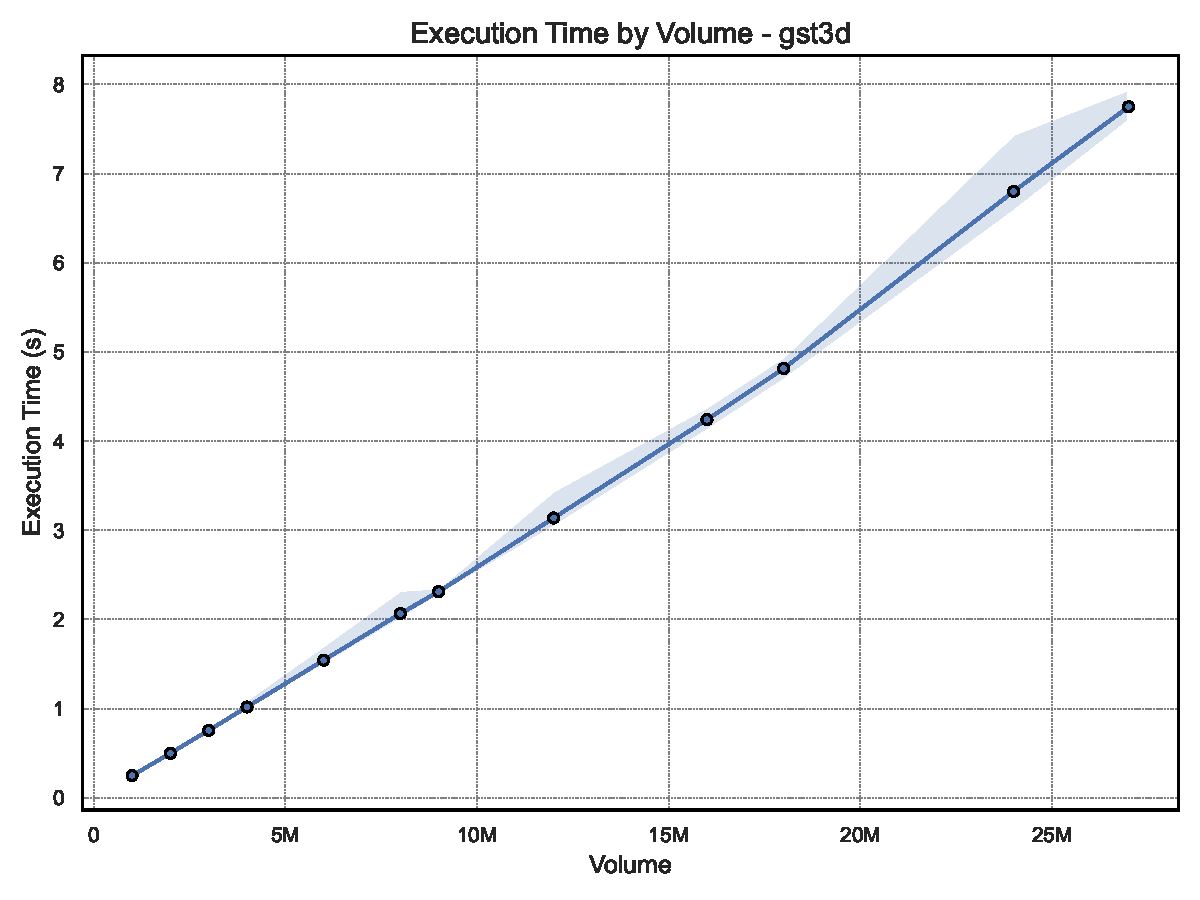
\includegraphics[width=\textwidth]{assets/images/05/execution_time_by_volume_gst3d}
    \end{subfigure}
    \hfill
    \begin{subfigure}[t]{0.49\textwidth}
        \centering
        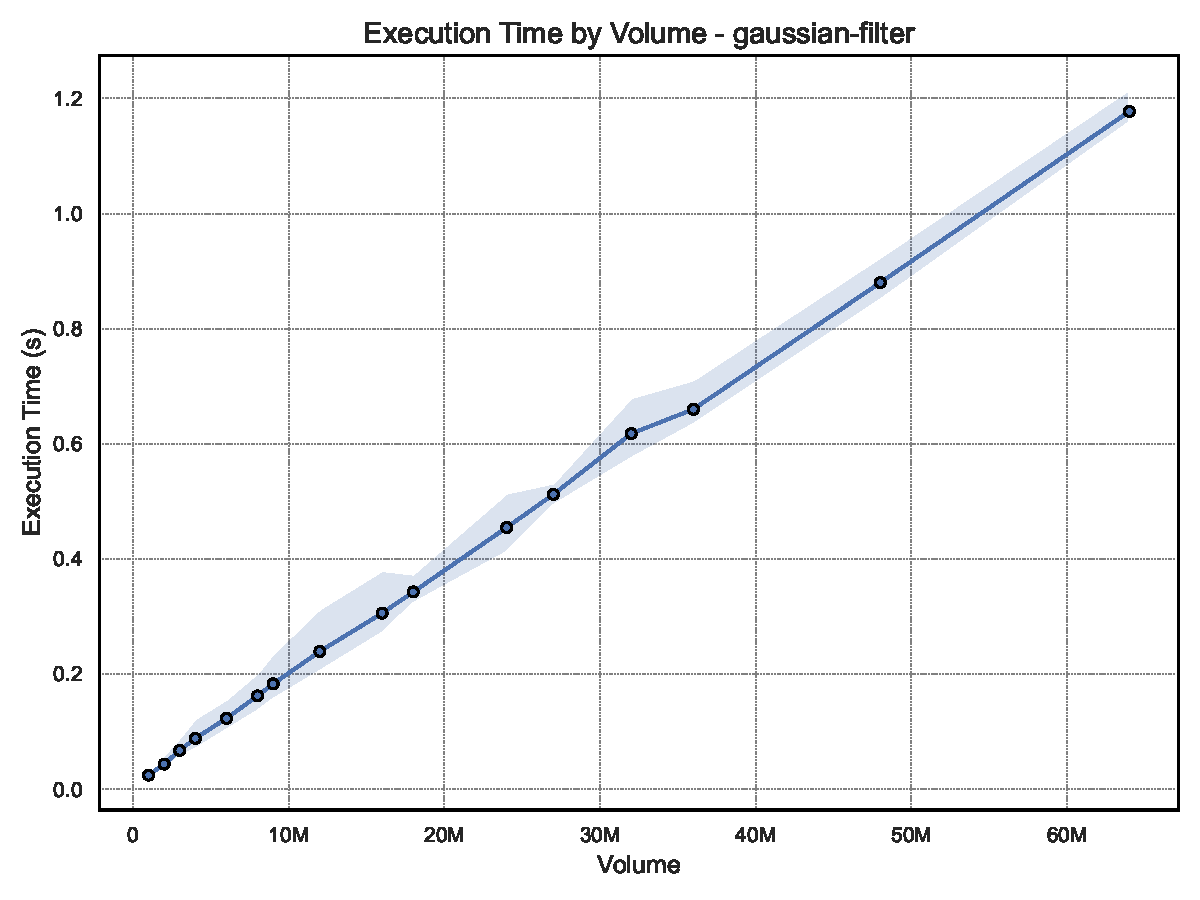
\includegraphics[width=\textwidth]{assets/images/05/execution_time_by_volume_gaussian-filter}
    \end{subfigure}
    \caption{
        Execution time by volume for Envelope, \ac{GST3D}, and Gaussian Filter. 
        All three operators show an increasing trend, reinforcing the impact of volume on processing duration. 
        \label{fig:execution_time_by_volume_facet}
    }
\end{figure*}

\subsection{Execution Time Distributions and Scaling Factor}
\label{subsec:execution-time-distributions-and-scaling}

To complement the volume-based analysis, Figures~\ref{fig:ex_peak_mu_facet}(a)--(b) compare execution time and peak memory usage across all operators.
Both metrics escalate in near-lockstep with input size.
Figure~\ref{fig:ex_peak_mu_facet}(c) then quantifies memory scaling slopes via linear-fits for each operator’s average peak \ac{RAM} usage. 
\EB{Acho que fica melhor mostrar o slope da regressão linear em uma tabela - você poderia mostrar o $R^2$ também. Isso tornadria o gráfico menor e talvez passível de inserção logo após o parágrafo que referencia ele.}
\ac{GST3D} stands out for having the highest slope, suggesting it holds more intermediate data structures during discontinuity detection.
Envelope lies in the middle, while Gaussian Filter’s slope is relatively smaller, implying that it processes data blocks \EBC{more incrementally}{o que quer dizer de forma mais incremental? seria por partes? Mas todos eles não realizam o cálculo por partes? i.e., por chunks?}.

\begin{figure*}[htbp]
    \centering
    \begin{subfigure}[t]{0.49\textwidth}
        \centering
        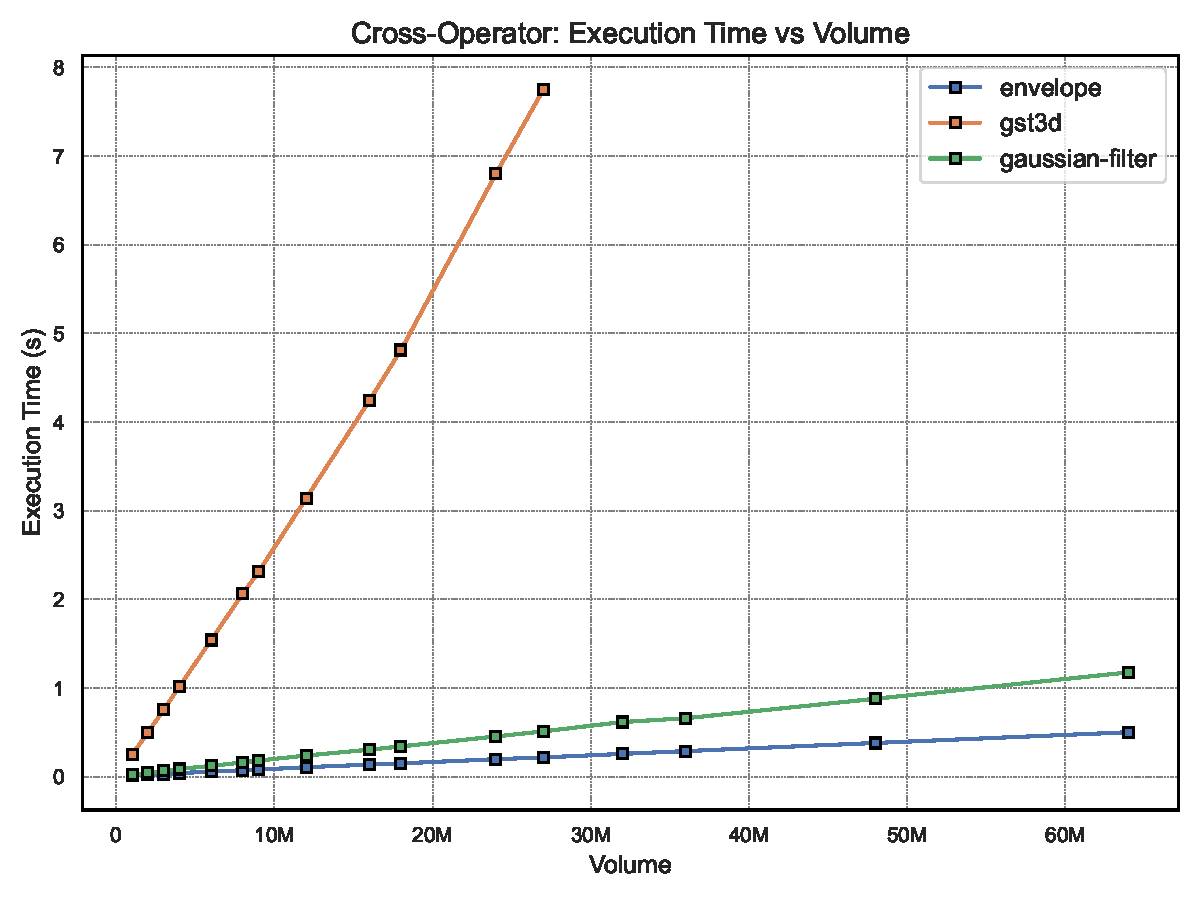
\includegraphics[width=\textwidth]{assets/images/05/cross_execution_time_by_volume}
        \caption{Execution time vs. volume for all three operators.}
    \end{subfigure}
    \hfill
    \begin{subfigure}[t]{0.49\textwidth}
        \centering
        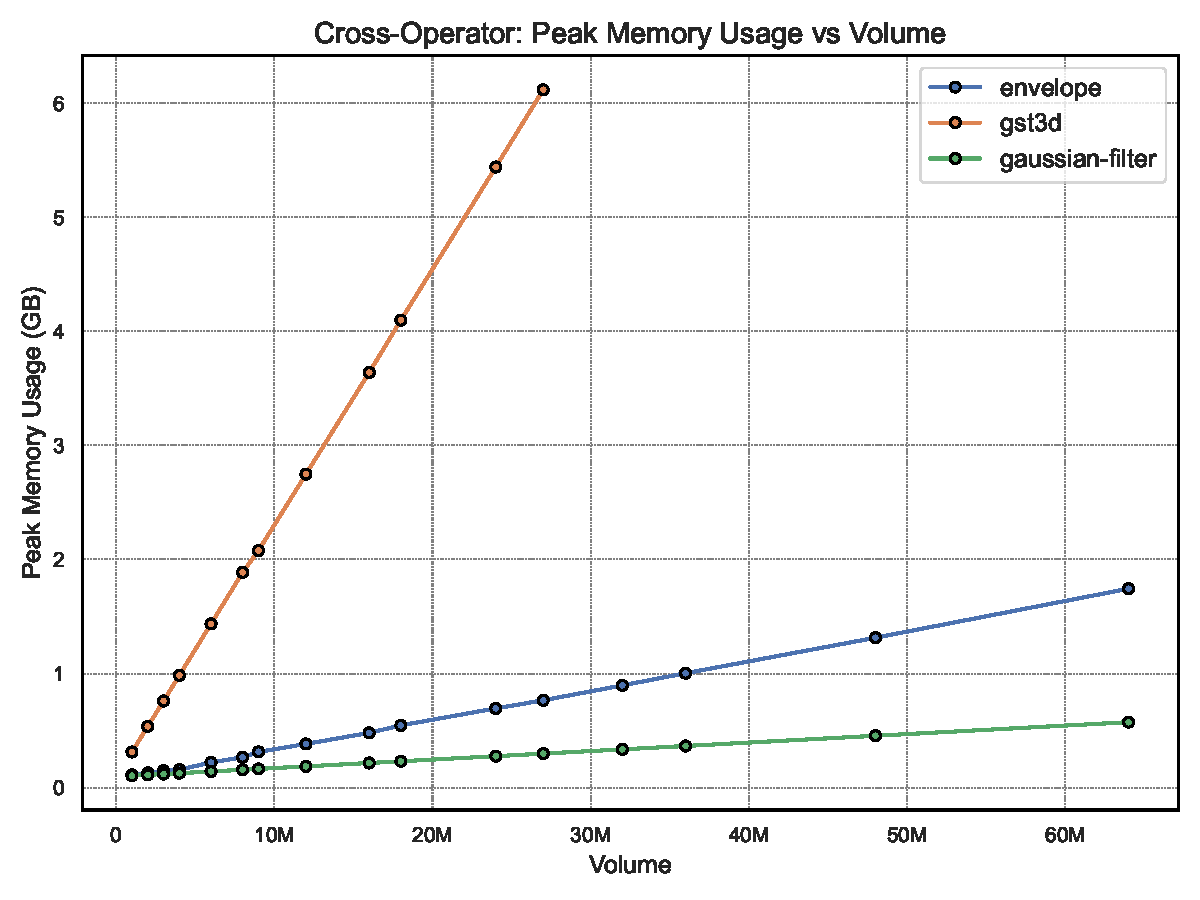
\includegraphics[width=\textwidth]{assets/images/05/cross_peak_memory_by_volume}
        \caption{Peak memory usage vs. volume for all three operators.}
    \end{subfigure}
    \hfill
    \begin{subfigure}[t]{0.49\textwidth}
        \centering
        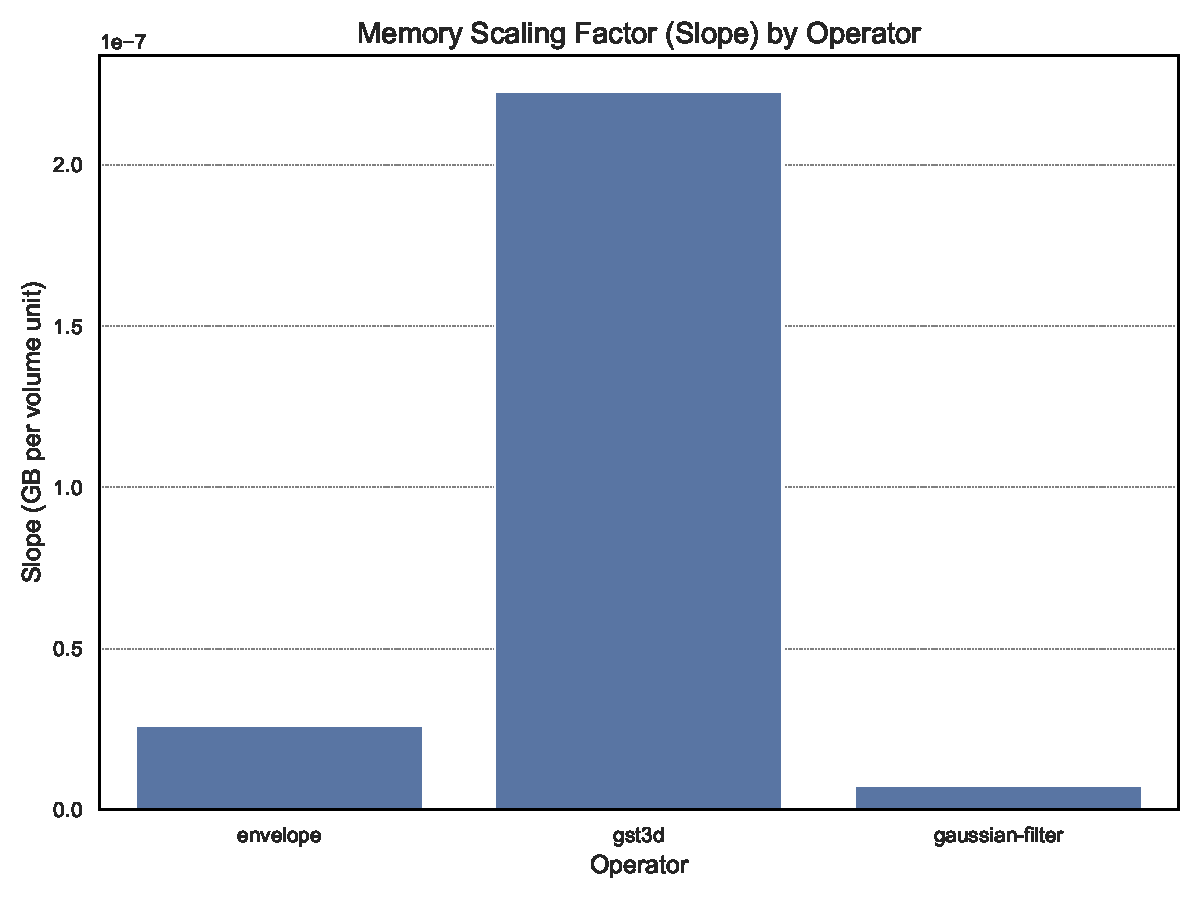
\includegraphics[width=\textwidth]{assets/images/05/cross_operator_memory_scaling_factor}
        \caption{
            Linear-fit slope values (GB/volume). Higher values indicate more pronounced memory growth.
            \EB{Como coloquei no texto, talvez fique melhor remover este gráfico daqui e colocar a informação em uma tabela.}
        }
    \end{subfigure}
    \caption{Combined view of execution time and peak memory usage by volume, and a bar chart revealing the linear-fit slopes for Envelope, \ac{GST3D}, and Gaussian Filter. \ac{GST3D} uses memory most aggressively, while Gaussian Filter is comparatively more memory efficient.}
    \label{fig:ex_peak_mu_facet}
\end{figure*}

In addition, the run durations exhibit right-skewed behavior (Figure~\ref{fig:execution_time_distribution_facet}), consistent with gamma- or lognormal-like distributions. \EB{Este gráfico mostra o histograma do tempo de execução de todos os experimentos? Variando o tamanho do dado? Se sim, a distribuição de tempo de execução tem uma relação mais forte com a seleção das amostras (tamanhos) do que com ruído no sistema, certo?}
While most executions concentrate in the lower range, occasional runs can be significantly longer.
Such tails are not unexpected in \ac{HPC} environments, where system-level noise or particular dataset structures can cause prolonged I/O or memory allocation overhead.
\EB{Não está claro pra mim como este gráfico e estes resultados de tempo contribuem para as principais conclusões derivadas neste capítulo. É interessante ter uma noção do tempo de execução, até mesmo para saber o custo de ser realizar estes experimentos e/ou coletar dados para treinar os modelos, mas além deste ponto, não sei se uma análise de correlação de features e/ou consumo de memória com o tempo de execução está dando suporte aos principais argumentos ou poluindo o capítulo.}

\begin{figure*}[htbp]
    \centering
    \begin{subfigure}[t]{0.49\textwidth}
        \centering
        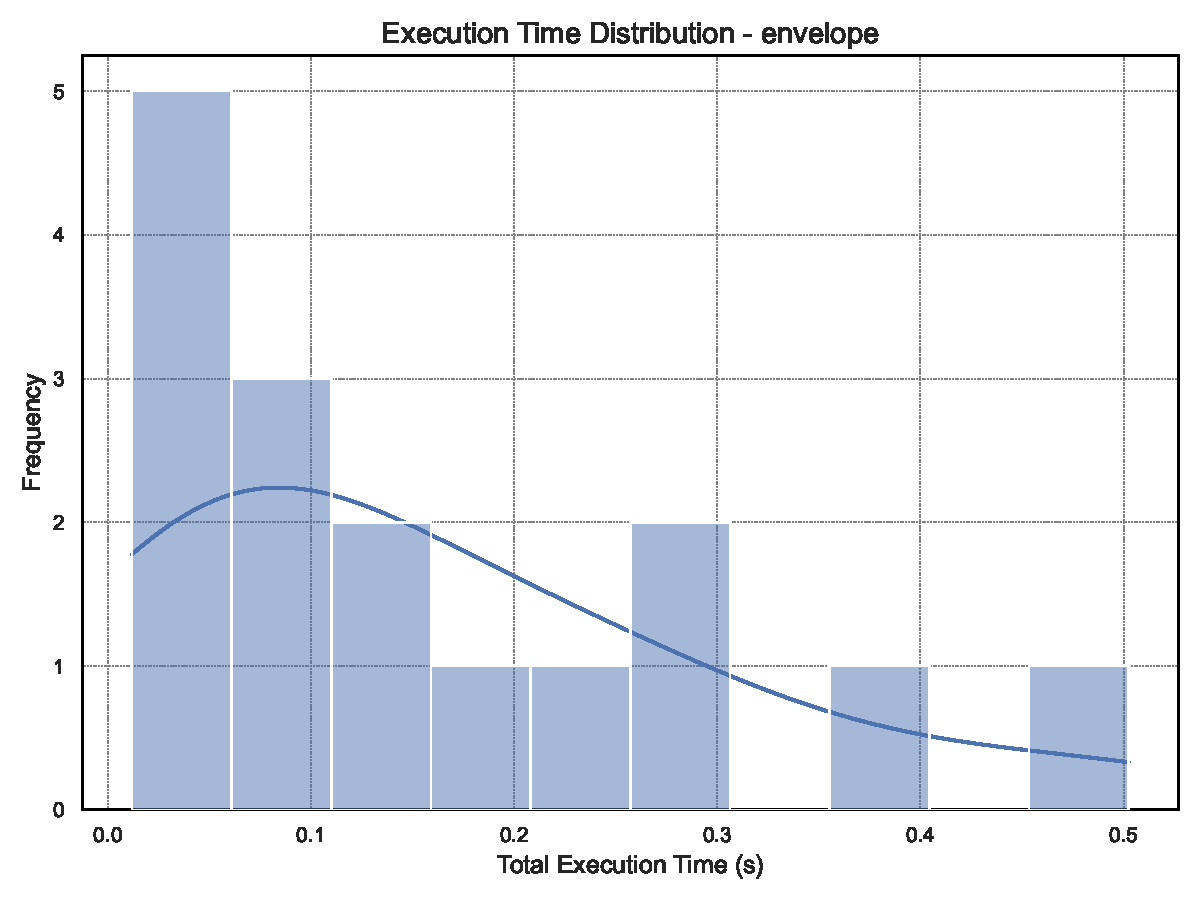
\includegraphics[width=\textwidth]{assets/images/05/execution_time_distribution_envelope}
    \end{subfigure}
    \hfill
    \begin{subfigure}[t]{0.49\textwidth}
        \centering
        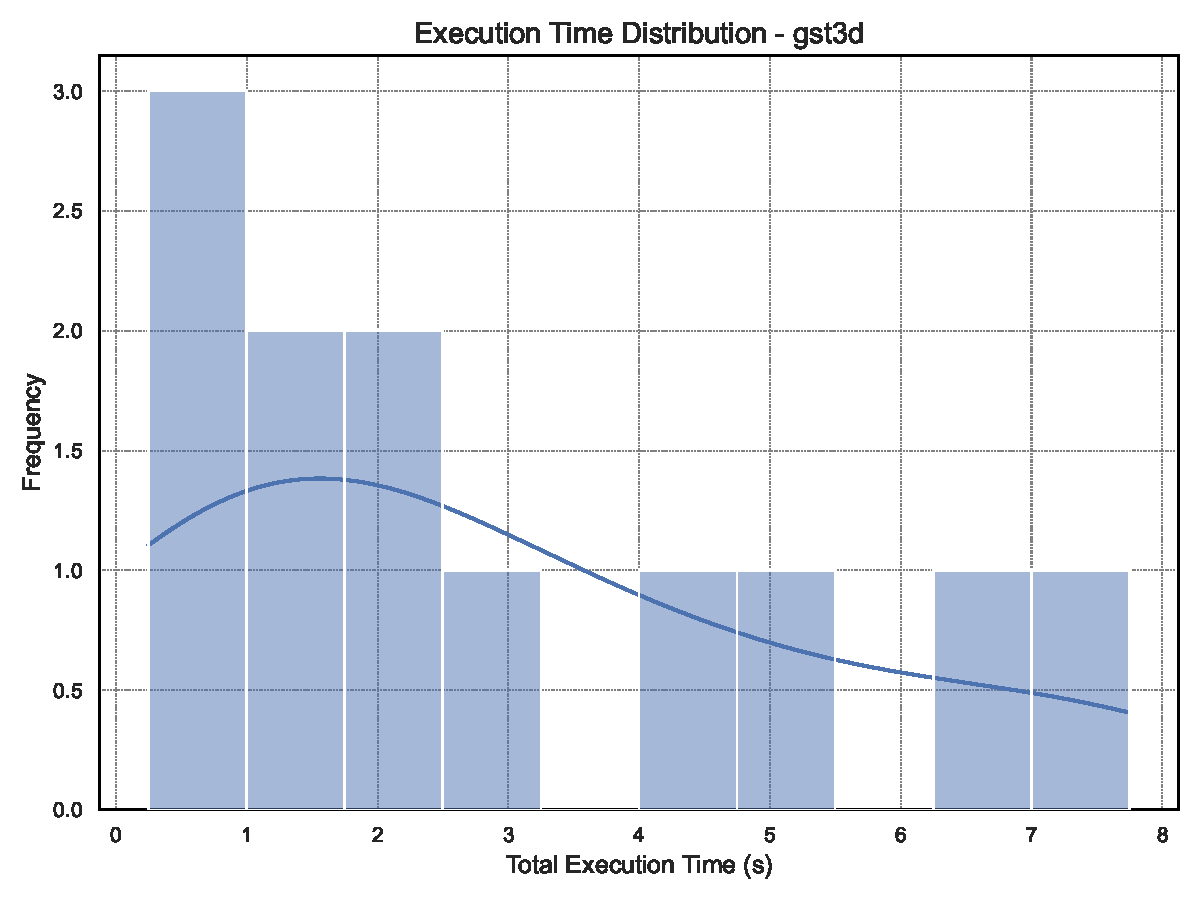
\includegraphics[width=\textwidth]{assets/images/05/execution_time_distribution_gst3d}
    \end{subfigure}
    \hfill
    \begin{subfigure}[t]{0.49\textwidth}
        \centering
        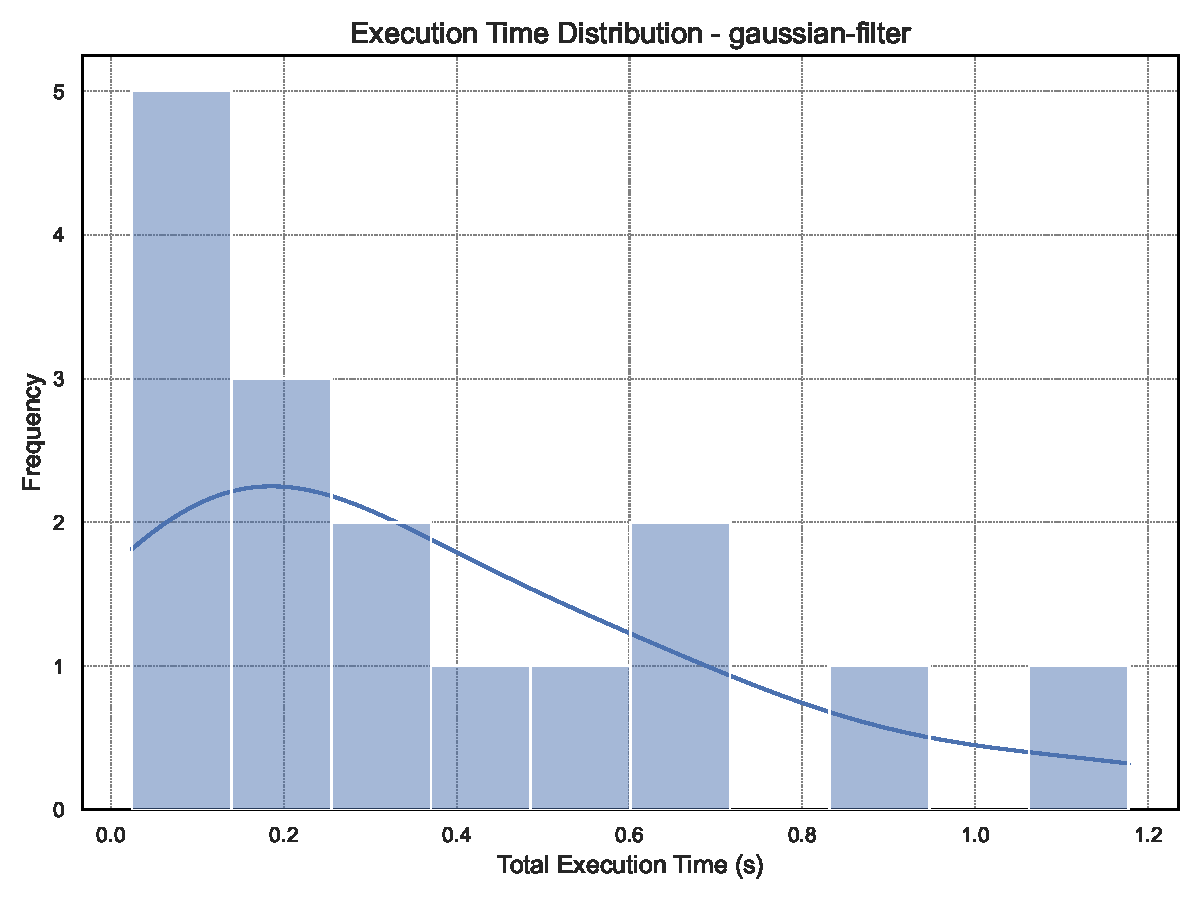
\includegraphics[width=\textwidth]{assets/images/05/execution_time_distribution_gaussian-filter}
    \end{subfigure}
    \caption{Execution time distributions for Envelope, \ac{GST3D}, and the Gaussian Filter. Each distribution displays a heavy right tail, indicating that while most runs finish quickly, certain configurations or system conditions can cause notable slowdowns.}
    \label{fig:execution_time_distribution_facet}
\end{figure*}

\subsection{Dimension-Specific and Time-Progression Analysis}
\label{subsec:dimension-specific-and-time-progression-analysis}

\EB{Como mencionei anteriormente, não está claro para mim se esta análise de tempo de execução é muito relevante.}

To better understand how different axes of the seismic volume factor into resource usage, we break down memory usage by \emph{inlines}, \emph{xlines}, and \emph{samples} for the Envelope operator~(Figure~\ref{fig:memory_usage_by_configuration_envelope}).
We observe that each dimension exerts a similar influence on memory consumption; no single dimension overwhelmingly dominates the Envelope’s consumption pattern.
This outcome aligns with the notion that Envelope is an element-wise amplitude calculation, depending uniformly on the size of the entire input array.

\begin{figure*}[htbp]
    \centering
    \begin{subfigure}[t]{0.49\textwidth}
        \centering
        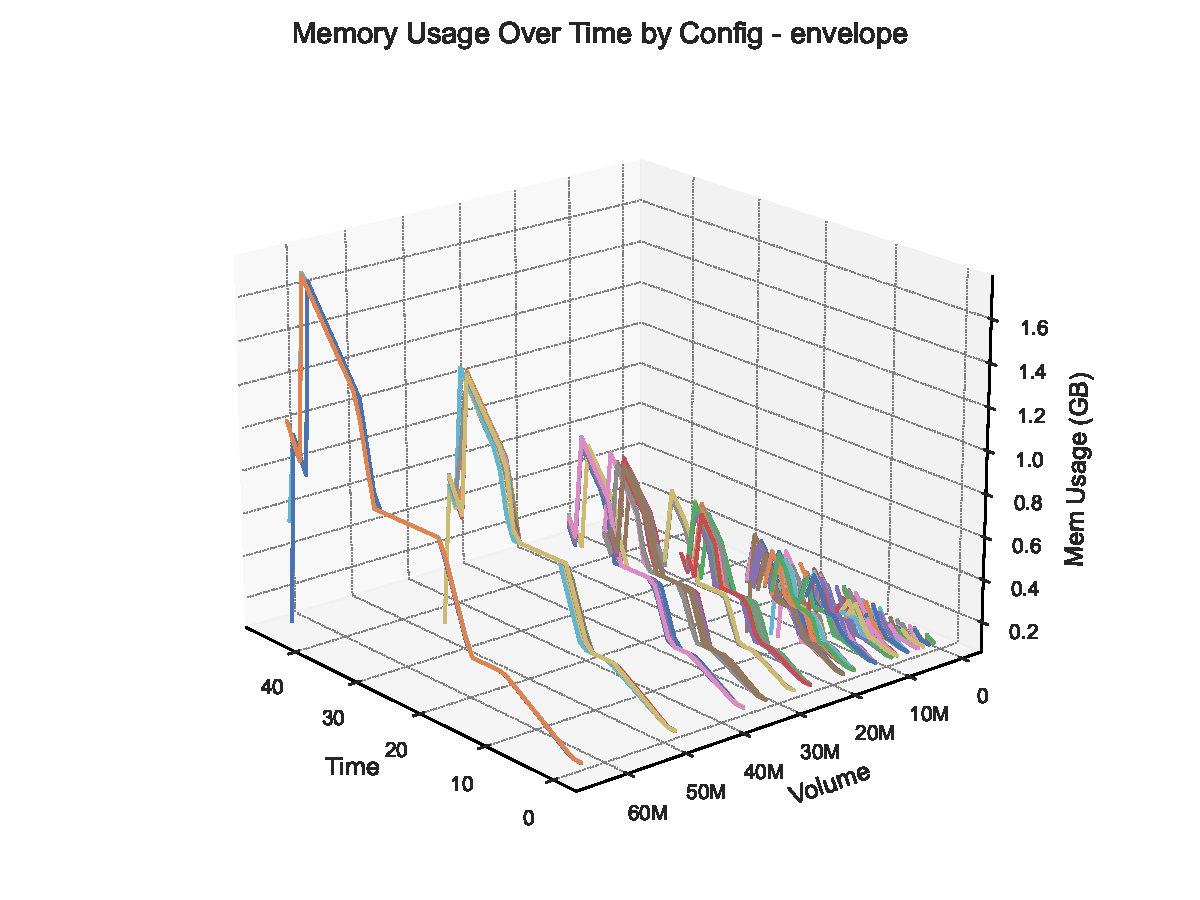
\includegraphics[width=\textwidth]{assets/images/05/memory_usage_by_configuration_envelope}
        \caption{Memory usage binned by individual shape parameters. Each axis increases overall memory similarly.}
    \end{subfigure}
    \hfill
    \begin{subfigure}[t]{0.49\textwidth}
        \centering
        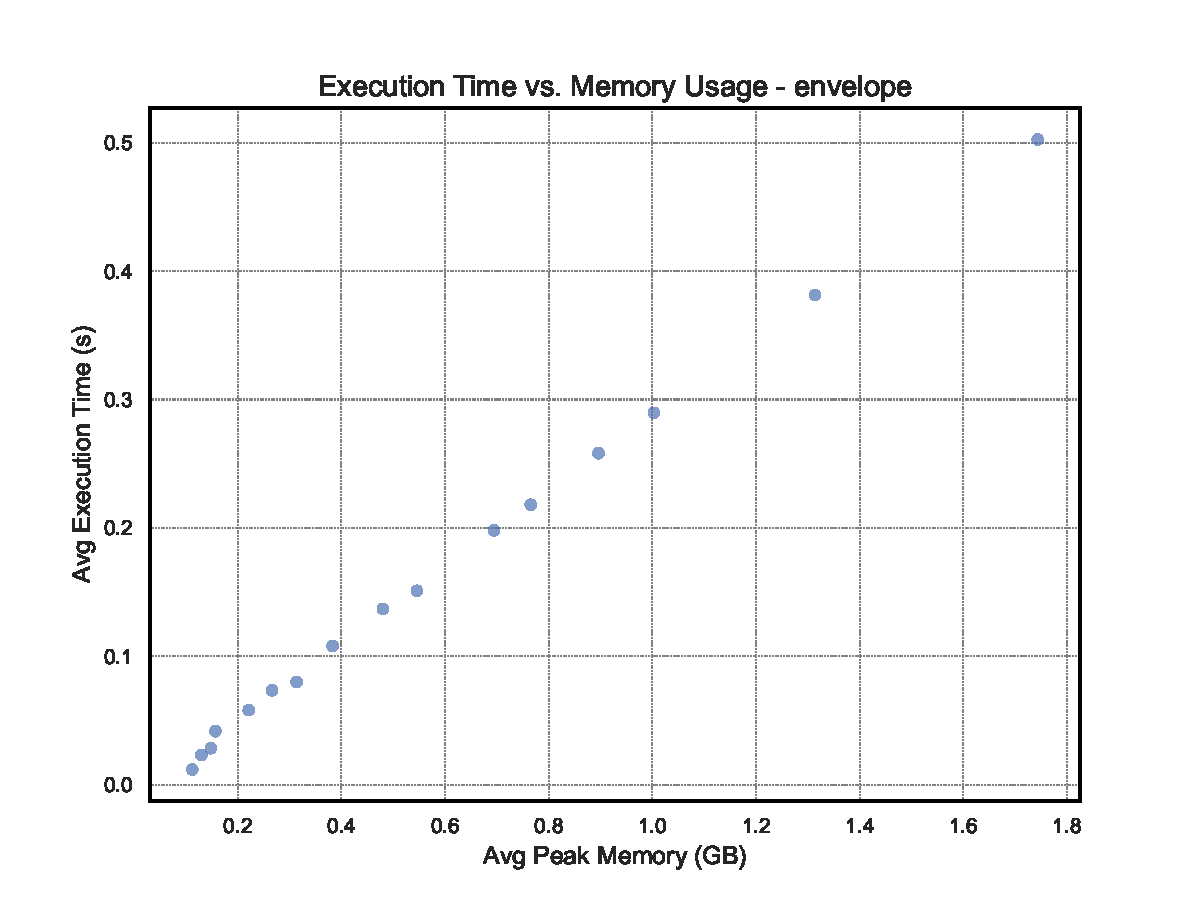
\includegraphics[width=\textwidth]{assets/images/05/execution_time_vs_memory_envelope}
        \caption{Execution time vs. memory usage for Envelope, indicating a mild correlation (longer runs often consume more \ac{RAM}).
            \EB{Não ficou claro para mim como este resultado dá suporte às principais conclusões do capítulo.}
        }
    \end{subfigure}
    \hfill
    \begin{subfigure}[t]{0.49\textwidth}
        \centering
        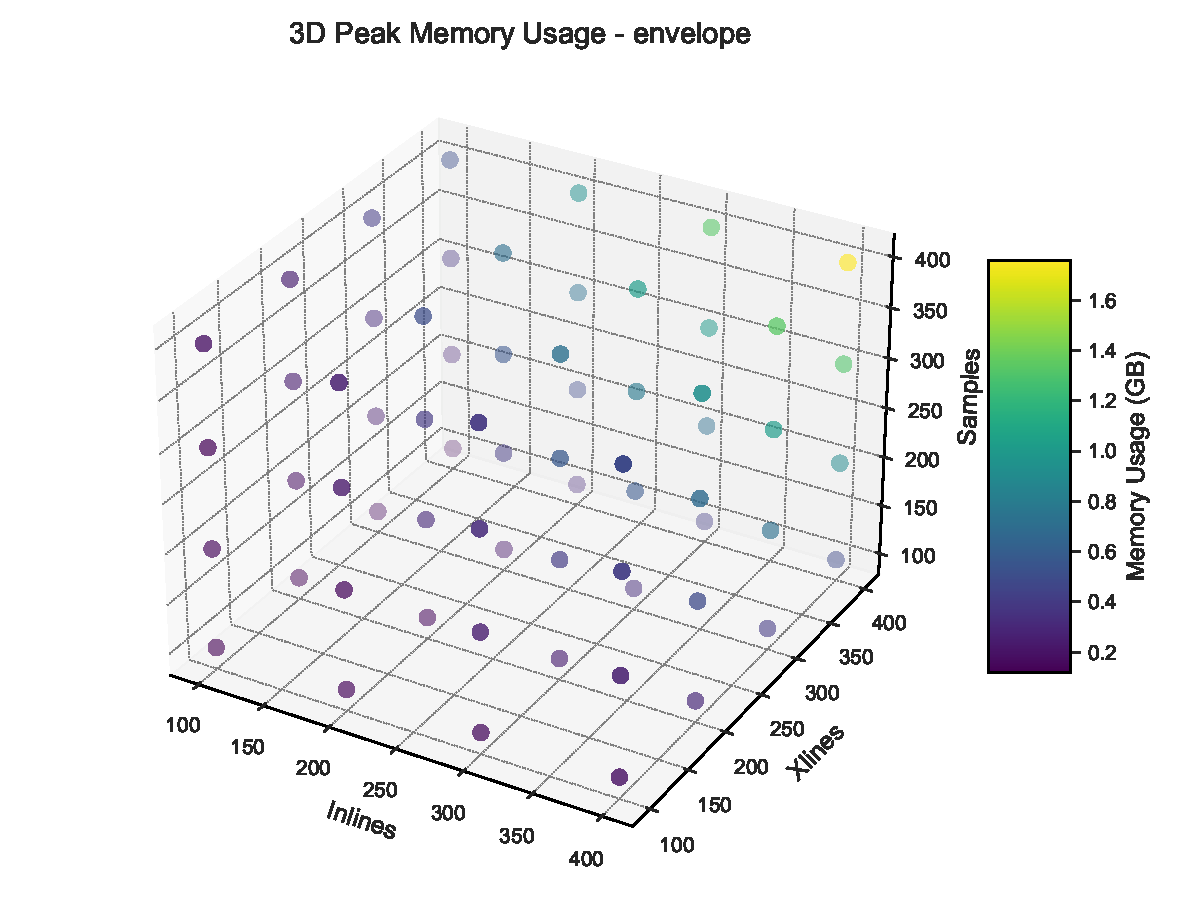
\includegraphics[width=\textwidth]{assets/images/05/memory_usage_inlines_xlines_samples_heatmap_envelope}
        \caption{Heatmap combining inlines, xlines, and samples into a 2D view; warmer colors indicate higher memory usage.
            \EB{Estou inferindo que o objetivo deste gráfico é mostrar que cada dimensão tem uma influência similar no consumo de memória. Se for o caso, acho que seria bom explicar o gráfico no texto e discutir quais características do gráfico levam a esta conclusão.}
        }
    \end{subfigure}
    \caption{Memory usage and runtime analysis for the Envelope operator. 
        All three dimensions appear to scale memory demand in a similar manner, and bigger shapes generally require longer processing times.
        \label{fig:memory_usage_by_configuration_envelope}
    }
\end{figure*}

Figure~\ref{fig:inline_xline_memory_usage_progression_envelope} further highlights how the Envelope operator’s memory usage accumulates over time.
The growth pattern is relatively uniform, aligning with the straightforward element-wise nature of the algorithm.
More complex operators like \ac{GST3D} may reveal steeper or stage-based ramps, particularly if certain algorithmic phases allocate additional buffers or caching mechanisms at specific intervals.
\EB{Qual a principal conclusão (\textit{insight}) que podemos derivar deste experimento?}

\begin{figure}[htbp]
    \centering
    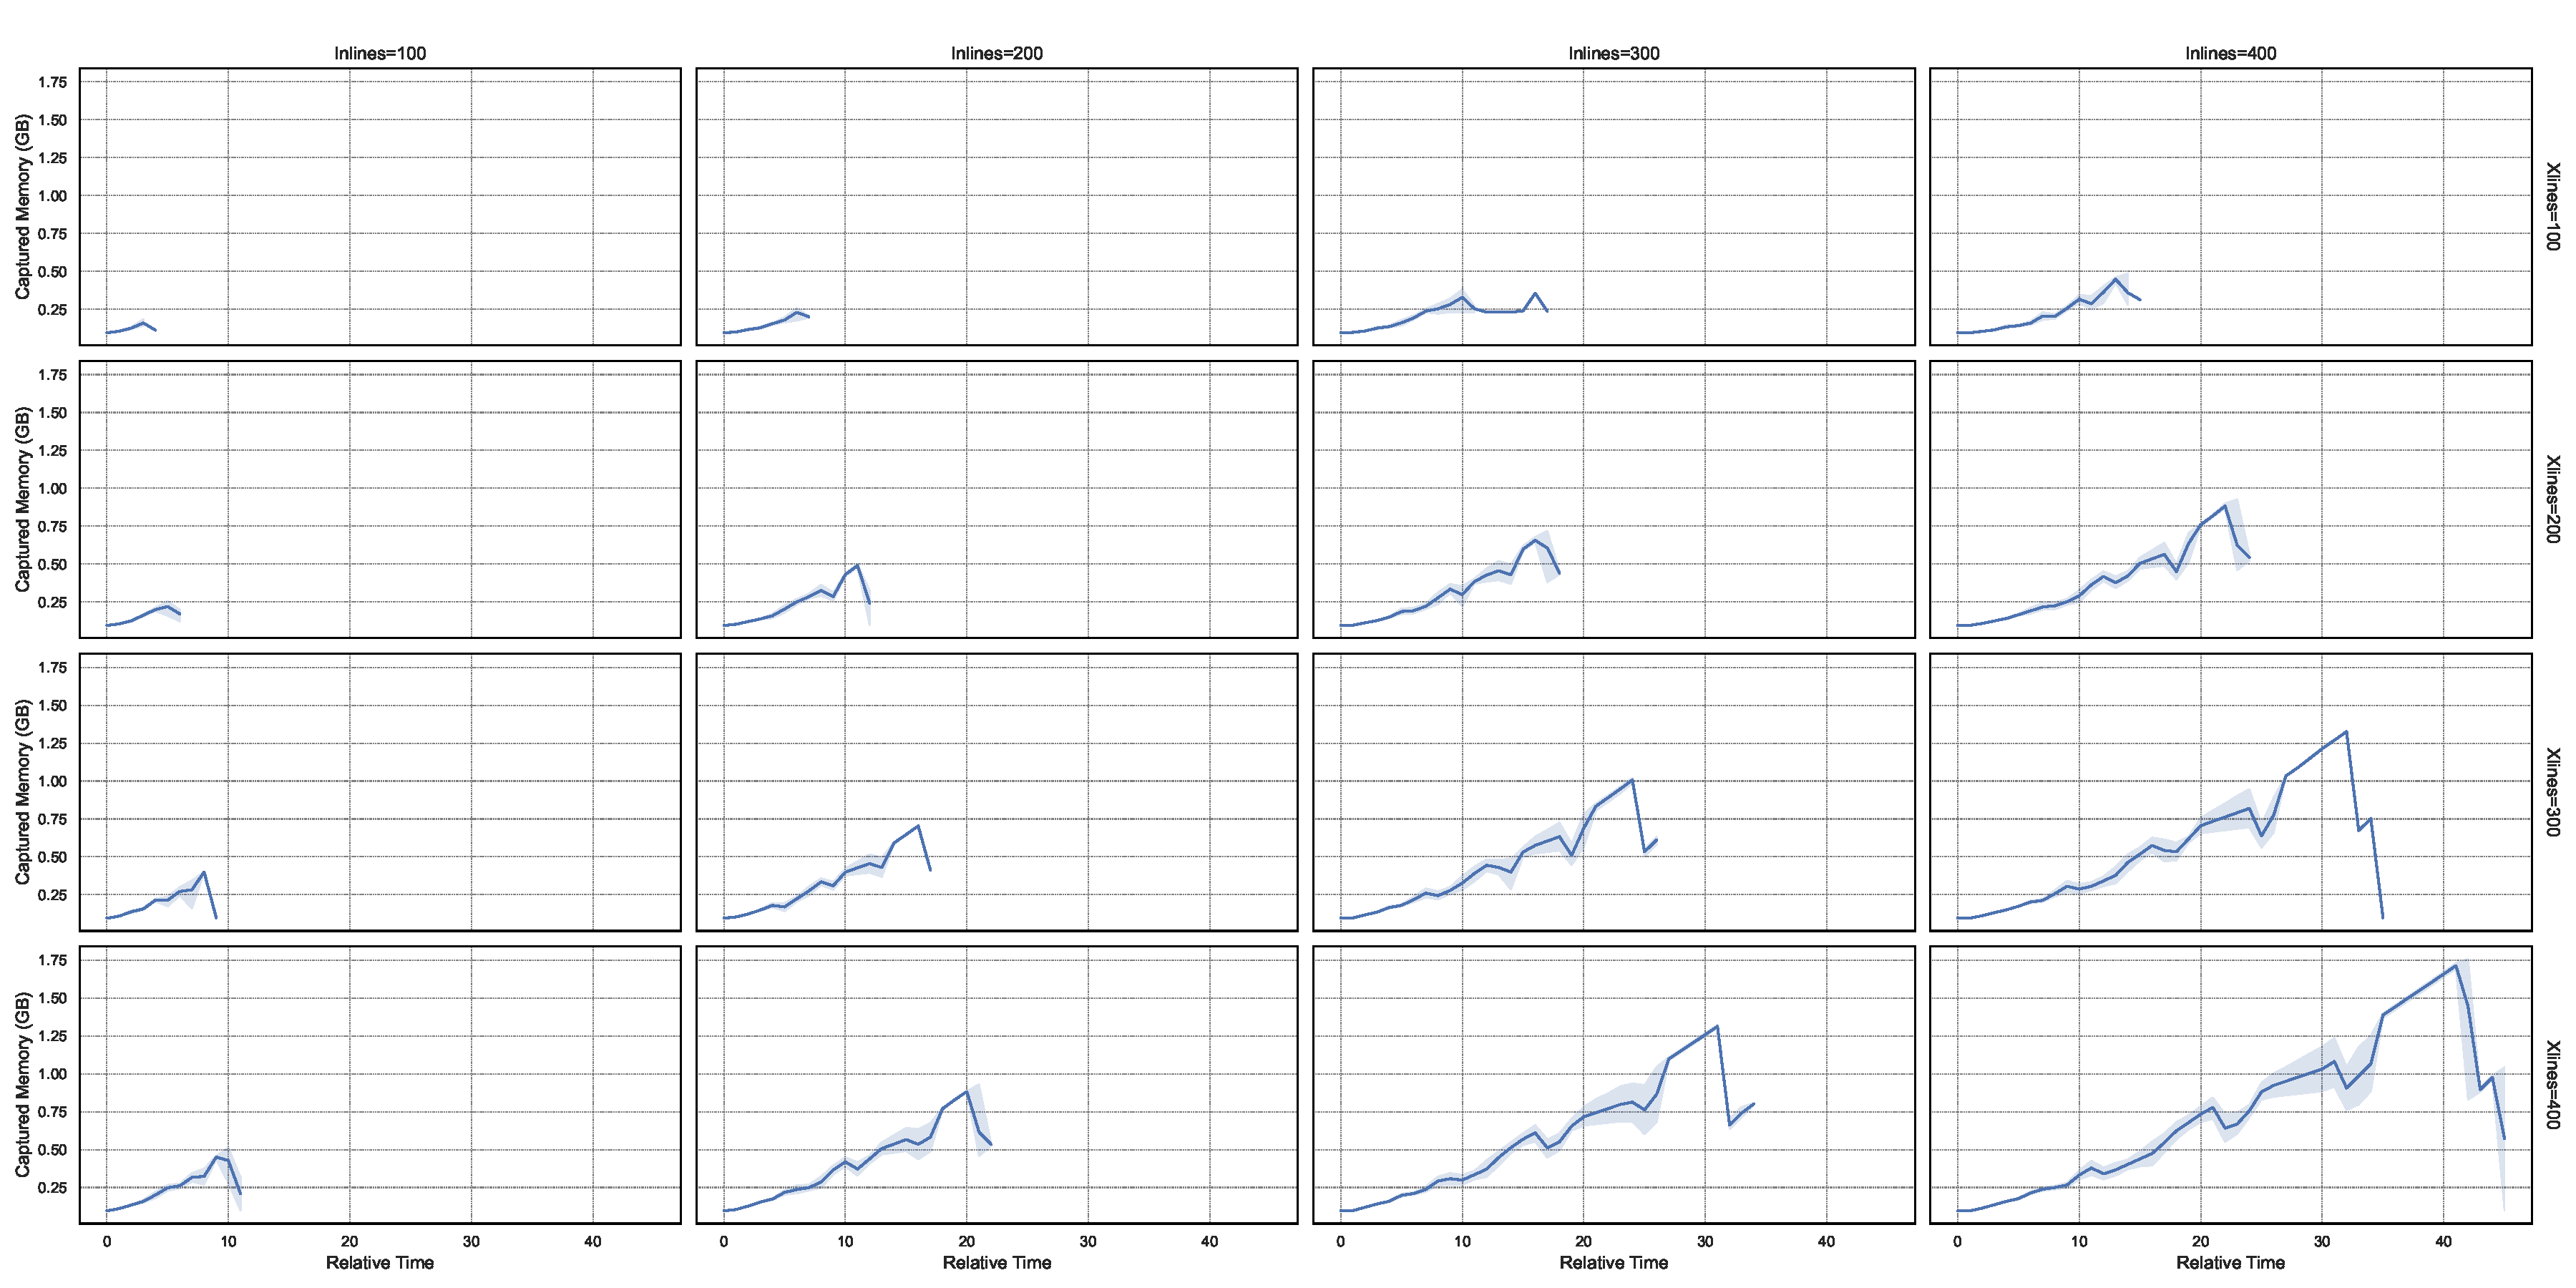
\includegraphics[width=\textwidth]{assets/images/05/inline_xline_memory_usage_progression_envelope}
    \caption{Memory usage progression over time (Envelope operator) for different inlines and xlines. 
        The consumption profile ramps up gradually rather than spiking in distinct phases.
        \label{fig:inline_xline_memory_usage_progression_envelope}
    }
\end{figure}

\subsection{Memory Safety Margins}
\label{subsec:memory-safety-margins}

In real-world \ac{HPC} contexts, underestimating memory can cause abrupt job failures, while overestimation wastes resources.
Figure~\ref{fig:memory_safety_margin} showcases how much peak usage can deviate from average usage by comparing mean and 95th-percentile values.
Envelope and \ac{GST3D} exhibit particularly large deviations for certain volume ranges, hinting that HPC practitioners may need to add a safety buffer beyond the mean consumption to accommodate transient memory spikes.
\EB{Este parágrafo me leva a crer que você está usando a \emph{feature} volume para fazer esta análise. Não seria mais adequado agrupar os dados de acordo com a tupla (inlines, xlines, samples) para evitar que variações de consumo de memória causadas por mudanças nestes valores nos levem a concluir que o motivo é o sistema? P.ex., a tupla (10, 10, 20) pode gerar resultados da tupla (20, 10, 10) que, apesar de terem o mesmo volume, são diferentes.}
\EB{Se tem tanta variação, como foi possível treinar os modelos somente com esta feature e chegar a valores de erro tão pequenos? Os erros não deveriam refletir as variações que observamos aqui?}


\begin{figure*}[htbp]
    \centering
    \begin{subfigure}[t]{0.49\textwidth}
        \centering
        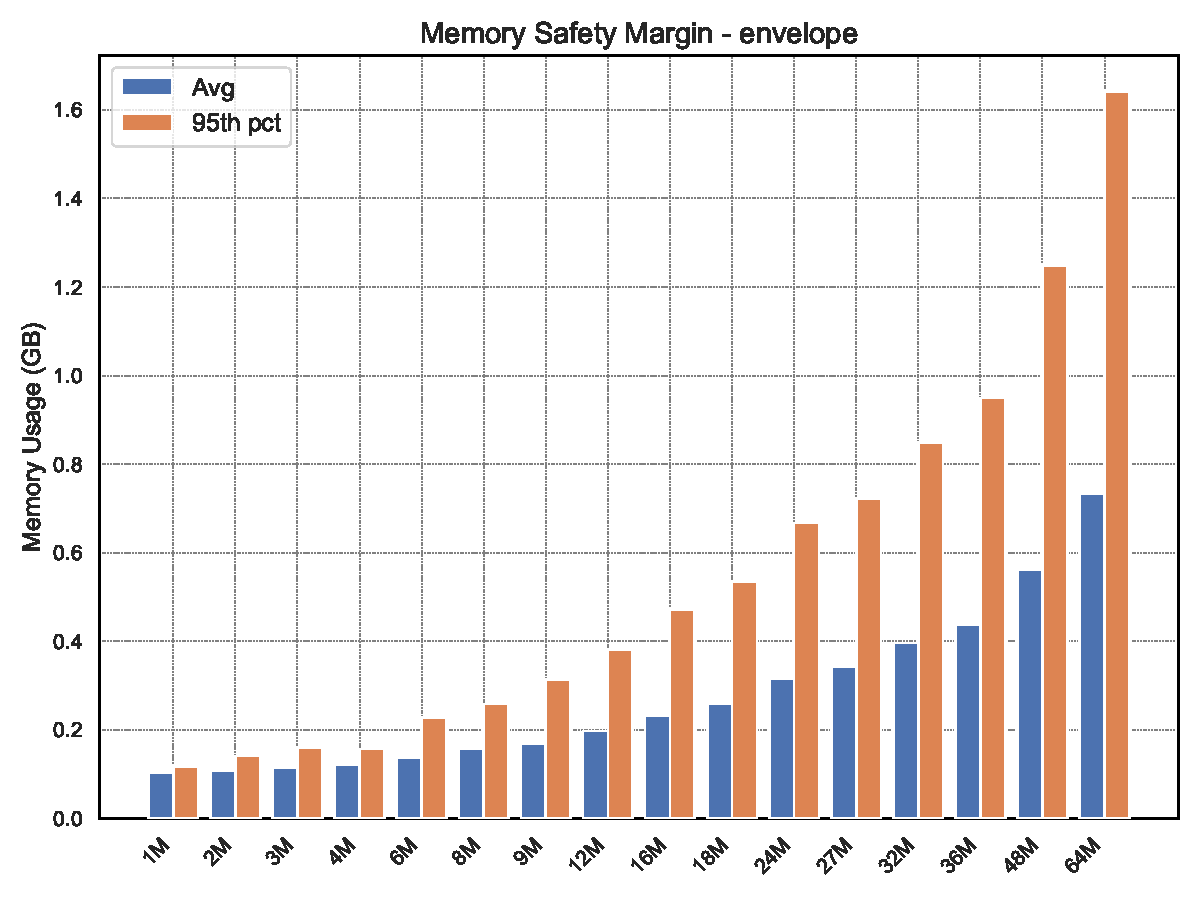
\includegraphics[width=\textwidth]{assets/images/05/memory_safety_margin_envelope}
    \end{subfigure}
    \hfill
    \begin{subfigure}[t]{0.49\textwidth}
        \centering
        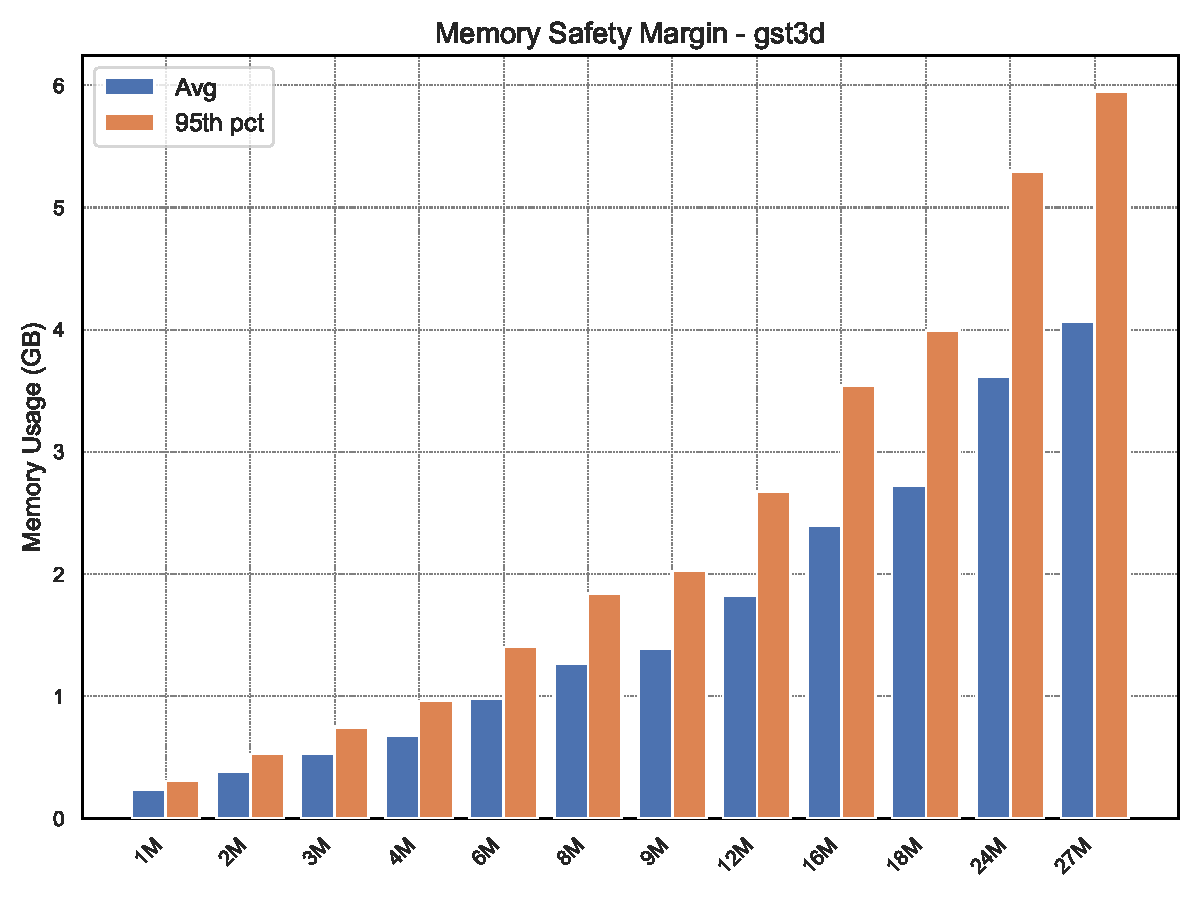
\includegraphics[width=\textwidth]{assets/images/05/memory_safety_margin_gst3d}
    \end{subfigure}
    \hfill
    \begin{subfigure}[t]{0.49\textwidth}
        \centering
        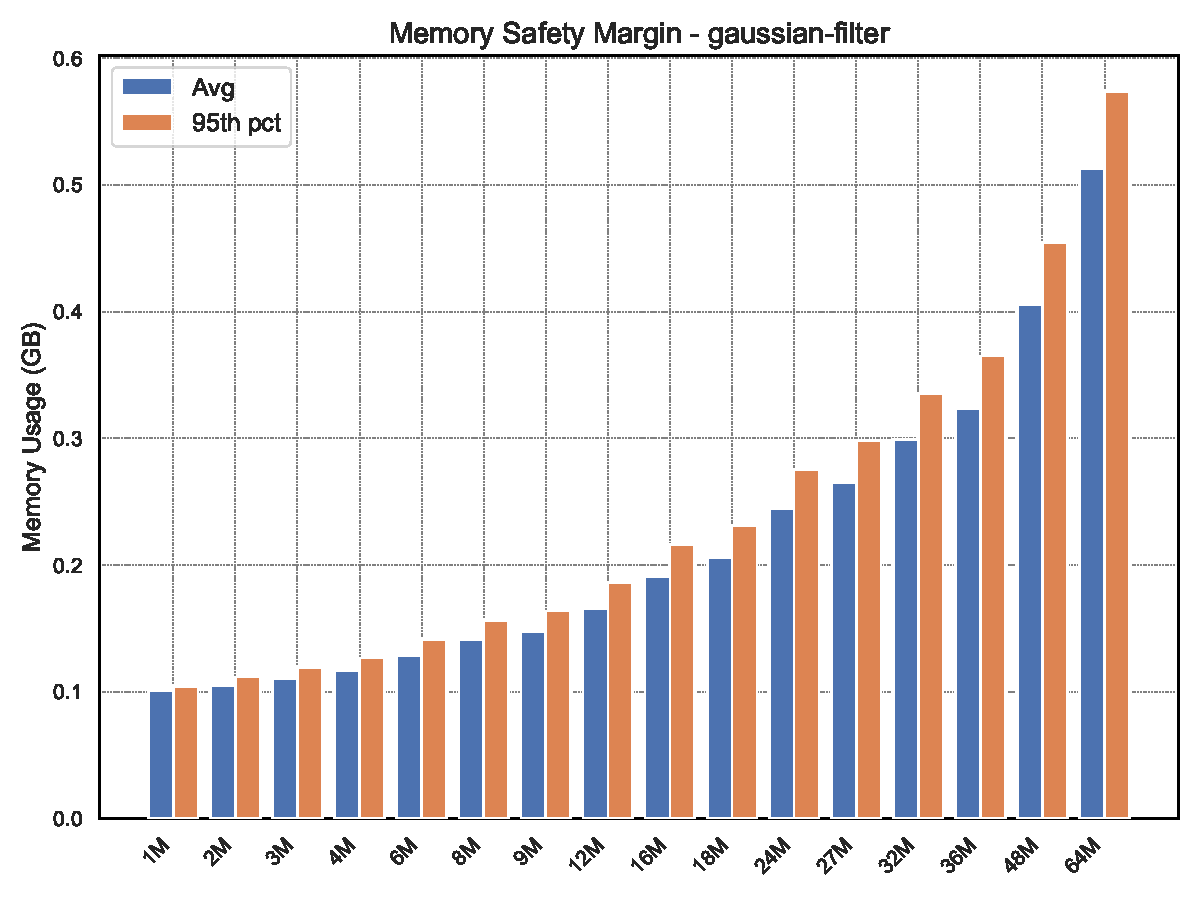
\includegraphics[width=\textwidth]{assets/images/05/memory_safety_margin_gaussian-filter}
    \end{subfigure}
    \caption{Memory safety margins for Envelope, \ac{GST3D}, and the Gaussian Filter. The 95th-percentile often surpasses mean usage by a noticeable margin, revealing the unpredictability of peak memory events.}
    \label{fig:memory_safety_margin}
\end{figure*}

These outliers can arise from transient allocation bursts, system-level scheduling, or overhead fluctuations.
Even with container-based isolation, kernel-level memory management can introduce sporadic spikes.
Recognizing these high-percentile events is critical for designing robust pre-runtime memory estimators.
If left unaccounted for, such transient peaks could lead to underestimation, especially for borderline volumes.

\EB{Este me parece ser uma seção bem importante, já que ela discute a questão da margem de erro que devemos levar em consideração na avaliação dos modelos. Quando trabalhamos com os modelos estamos utilizando dados baseados na média ou no 95\%?} 
\EB{Para refletir: Será que não deveríamos estar usando os dados crus, e monitorar estas variações nos errors?}

\EB{BTW, esta variabilidade é usada no cálculo do score que você menciona nas seções subsequentes?}

\subsection{Dimension Correlations}
\label{subsec:dimension-correlations}

We can further investigate how dimension-specific growth patterns contribute to overall memory usage by plotting pairwise relationships between memory usage and the three shape parameters.
Figure~\ref{fig:memory_vs_dimensions_pairplot_gst3d} shows that \ac{GST3D}, in particular, has strong positive correlations between each dimension and peak memory.
Meanwhile, dimension--dimension scatter plots sometimes show inverse correlations due to the systematic way shapes were varied (when one axis is large, another might be slightly smaller).
Nevertheless, once all three dimensions expand simultaneously, the net memory usage grows sharply.

\EB{Daniel, não entendi o gráfico. O que significam os pontos azuis e as linhas vermelhas?}

\begin{figure}[htbp]
    \centering
    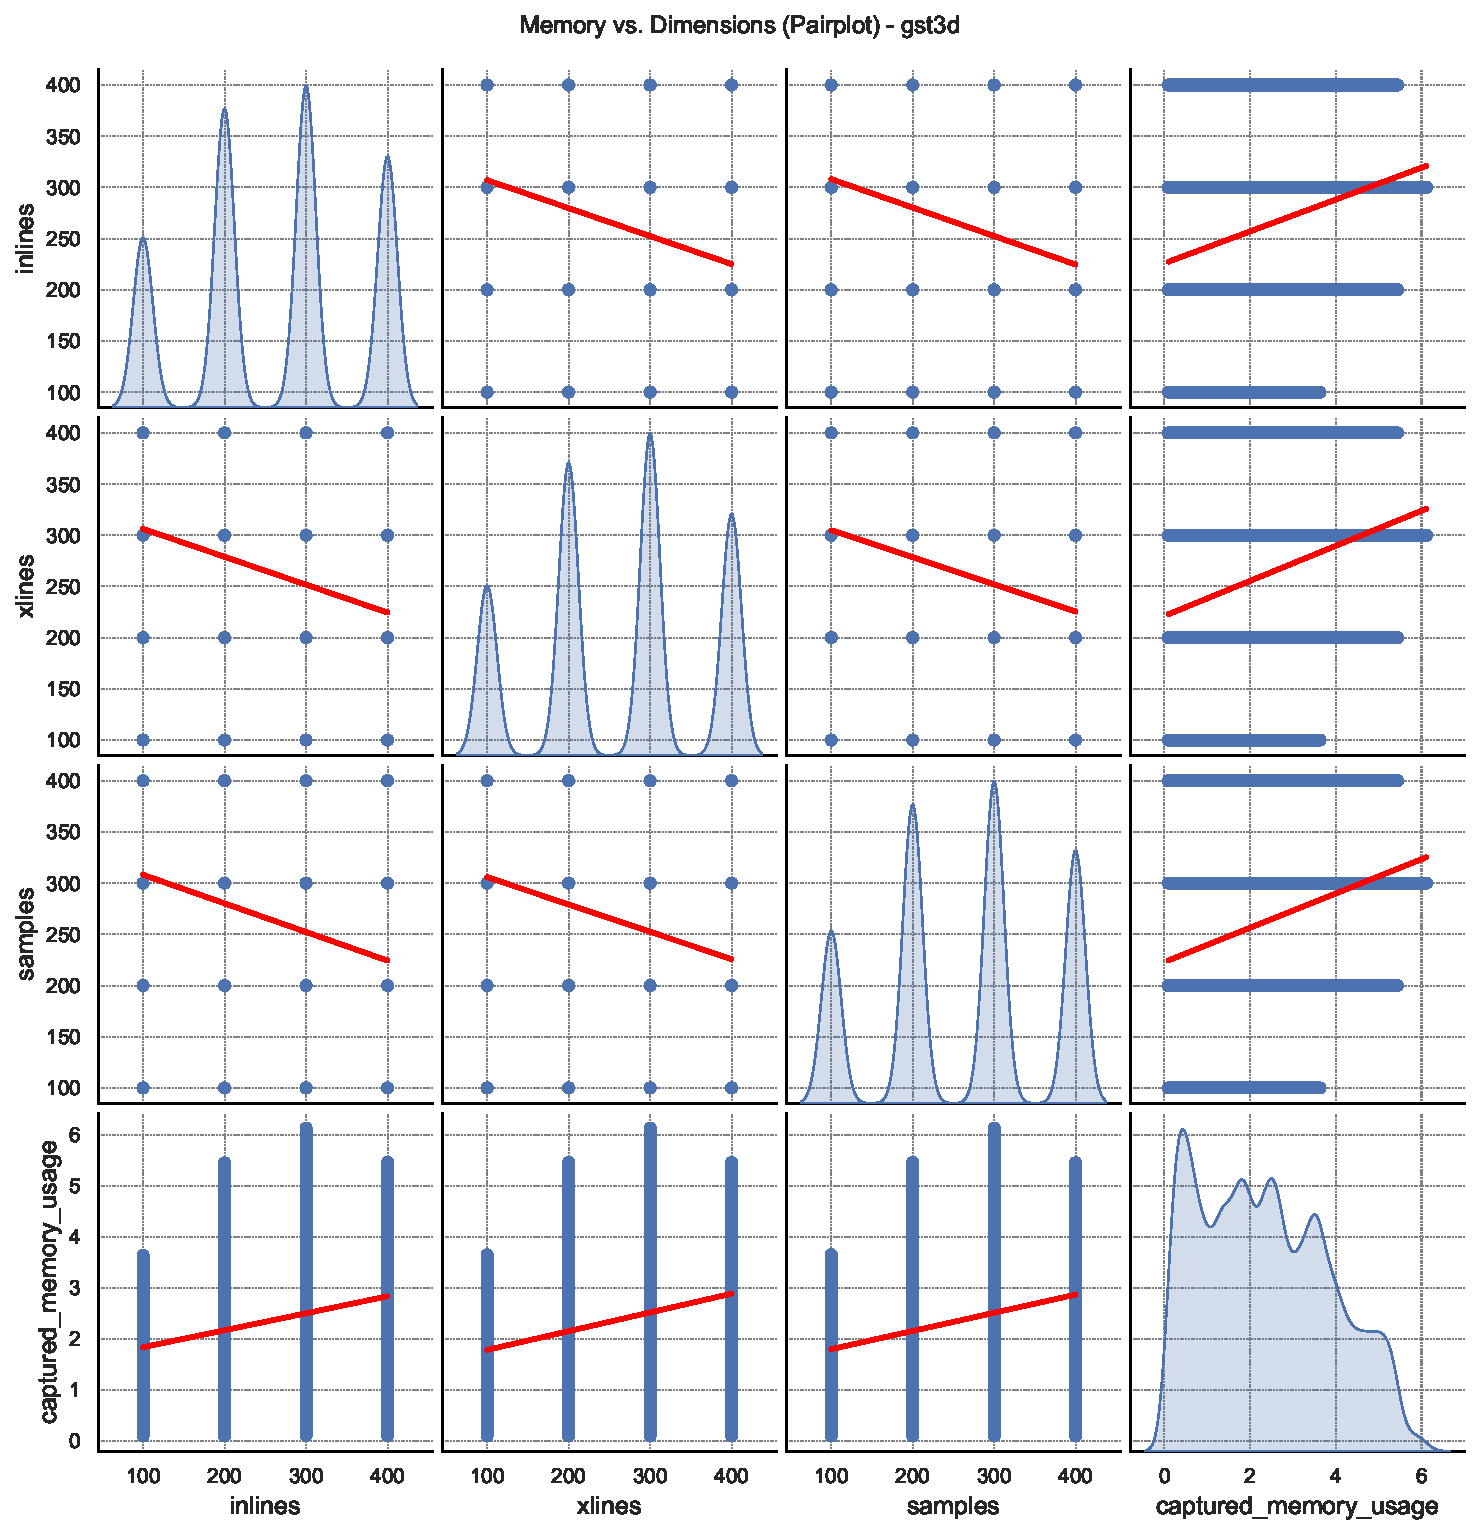
\includegraphics[width=0.9\textwidth]{assets/images/05/memory_vs_dimensions_pairplot_gst3d}
    \caption{Pairplot for \ac{GST3D} memory usage against inlines, xlines, and samples. Positive slopes in memory-related plots confirm that larger shape parameters escalate the overall memory footprint.}
    \label{fig:memory_vs_dimensions_pairplot_gst3d}
\end{figure}

These pairwise correlations, combined with the linear volume trend, underscore that each dimension matters and that polynomial or interaction-based features can help capture how memory usage evolves in less trivial cases (e.g., operators whose complexity grows nonlinearly along certain axes).
\EB{Não ficou claro para mim como você chegou nesta conclusão.}

\subsection{Summary of Observed Resource Usage}
\label{subsec:resource-usage-summary}

Table~\ref{tab:operator_summary_aggregates} provides a high-level summary of all tested volume ranges, memory usage spans, and measured execution times for each operator.
It highlights how, for similarly sized volumes, \ac{GST3D} consistently demands the greatest \EBADD{amount of} \ac{RAM}, with Envelope requiring intermediate amounts, and Gaussian Filter at the lower end (though still significant).
Processing times echo these patterns, with more complex or data-hungry operations tending to take longer.

\begin{table}[htbp]
    \centering
    \begin{tabular}{lcccc}
        \hline
        \textbf{Operator} & \textbf{Volume Range} & \textbf{Peak Mem. Usage (GB)} & \textbf{Exec. Time (s)} \\ \hline
        Envelope &
        $10^6 \!\to\! 6.4\times10^7$ &
        0.10 -- 1.76 &
        0.0106 -- 0.5025 \\
        \ac{GST3D} &
        $10^6 \!\to\! 2.7\times10^7$ &
        0.31 -- 6.12 &
        0.2475 -- 7.75 \\
        Gaussian Filter &
        $10^6 \!\to\! 6.4\times10^7$ &
        0.10 -- 0.57 &
        0.0232 -- 1.22 \\
        \hline
    \end{tabular}
    \caption{Resource usage summary for Envelope, \ac{GST3D}, and Gaussian Filter.
    Volumes are specified in number of elements (e.g., $100 \times 100 \times 100 = 10^6$).
    Memory usage is in GB and time is in seconds.
    Each range denotes the min and max observed across tested volumes.}
    \label{tab:operator_summary_aggregates}
\end{table}

In general, both memory and runtime grow at a near-linear rate, reinforcing the fundamental role of volume in resource demands.
These findings suggest that shape-driven models are likely to be quite effective, especially if they incorporate slight nonlinearities or additional features to handle outliers.
The next sections \EBRPD{delve into}{discuss} how these raw measurements translate into model predictions, discussing which methods and features best capture the trends and variability described above.
